%%%%%%%%%%%%%%%%%%%%%%%%%%%%%%%%%%%%%%%%
% datoteka diploma-FRI-vzorec.tex
%
%POZOR: ta verzija ne producira pdf datoteke v pdf/A formatu!!!
%namenjena je le za nalogo pri Diplomskem seminarju!
%
% vzorčna datoteka za pisanje diplomskega dela v formatu LaTeX
% na UL Fakulteti za računalništvo in informatiko
%
% na osnovi starejših verzij vkup spravil Franc Solina, maj 2021
% prvo verzijo je leta 2010 pripravil Gašper Fijavž
%
% za upravljanje z literaturo ta vezija uporablja BibLaTeX
%
% svetujemo uporabo Overleaf.com - na tej spletni implementaciji LaTeXa ta vzorec zagotovo pravilno deluje
%

\documentclass[a4paper,12pt,openright]{book}
%\documentclass[a4paper, 12pt, openright, draft]{book}  Nalogo preverite tudi z opcijo draft, ki pokaže, katere vrstice so predolge! Pozor, v draft opciji, se slike ne pokažejo!
 
\usepackage[utf8]{inputenc}   % omogoča uporabo slovenskih črk kodiranih v formatu UTF-8
\usepackage[slovene,english]{babel}    % naloži, med drugim, slovenske delilne vzorce
\usepackage[pdftex]{graphicx}  % omogoča vlaganje slik različnih formatov
\usepackage{fancyhdr}          % poskrbi, na primer, za glave strani
\usepackage{amssymb}           % dodatni matematični simboli
\usepackage{amsmath}           % eqref, npr.
\usepackage{hyperxmp}
\usepackage[hyphens]{url}
\usepackage{csquotes}
\usepackage[pdftex, colorlinks=true,
						citecolor=black, filecolor=black, 
						linkcolor=black, urlcolor=black,
						pdfproducer={LaTeX}, pdfcreator={LaTeX}]{hyperref}

\usepackage{color}
\usepackage{soul}

\usepackage[
backend=biber,
style=numeric,
sorting=nty,
]{biblatex}


\addbibresource{sources.bib} %Imports bibliography file


%%%%%%%%%%%%%%%%%%%%%%%%%%%%%%%%%%%%%%%%
%	DIPLOMA INFO
%%%%%%%%%%%%%%%%%%%%%%%%%%%%%%%%%%%%%%%%
\newcommand{\ttitle}{Vizualno sledenje na vgrajenih napravah}
\newcommand{\ttitleEn}{Visual tracking on embedded devices}
\newcommand{\tsubject}{\ttitle}
\newcommand{\tsubjectEn}{\ttitleEn}
\newcommand{\tauthor}{Nik Prinčič}
\newcommand{\tkeywords}{računalniški vid na vgrajenih napravah, DepthAI, vizualni sledilnik}
\newcommand{\tkeywordsEn}{embedded computer vision, DepthAI, visual tracker}

%%%%%%%%%%%%%%%%%%%%%%%%%%%%%%%%%%%%%%%%
%	HYPERREF SETUP
%%%%%%%%%%%%%%%%%%%%%%%%%%%%%%%%%%%%%%%%
\hypersetup{pdftitle={\ttitle}}
\hypersetup{pdfsubject=\ttitleEn}
\hypersetup{pdfauthor={\tauthor}}
\hypersetup{pdfkeywords=\tkeywordsEn}

%%%%%%%%%%%%%%%%%%%%%%%%%%%%%%%%%%%%%%%%
% postavitev strani
%%%%%%%%%%%%%%%%%%%%%%%%%%%%%%%%%%%%%%%%  

\addtolength{\marginparwidth}{-20pt} % robovi za tisk
\addtolength{\oddsidemargin}{40pt}
\addtolength{\evensidemargin}{-40pt}

\renewcommand{\baselinestretch}{1.3} % ustrezen razmik med vrsticami
\setlength{\headheight}{15pt}        % potreben prostor na vrhu
\renewcommand{\chaptermark}[1]%
{\markboth{\MakeUppercase{\thechapter.\ #1}}{}} \renewcommand{\sectionmark}[1]%
{\markright{\MakeUppercase{\thesection.\ #1}}} \renewcommand{\headrulewidth}{0.5pt} \renewcommand{\footrulewidth}{0pt}
\fancyhf{}
\fancyhead[LE,RO]{\sl \thepage} 
%\fancyhead[LO]{\sl \rightmark} \fancyhead[RE]{\sl \leftmark}
\fancyhead[RE]{\sc \tauthor}              % dodal Solina
\fancyhead[LO]{\sc Diplomska naloga}     % dodal Solina


\newcommand{\BibLaTeX}{{\sc Bib}\LaTeX}
\newcommand{\BibTeX}{{\sc Bib}\TeX}

%%%%%%%%%%%%%%%%%%%%%%%%%%%%%%%%%%%%%%%%
% naslovi
%%%%%%%%%%%%%%%%%%%%%%%%%%%%%%%%%%%%%%%%  

\newcommand{\autfont}{\Large}
\newcommand{\titfont}{\LARGE\bf}
\newcommand{\clearemptydoublepage}{\newpage{\pagestyle{empty}\cleardoublepage}}
\setcounter{tocdepth}{1}	      % globina kazala

%%%%%%%%%%%%%%%%%%%%%%%%%%%%%%%%%%%%%%%%
% konstrukti
%%%%%%%%%%%%%%%%%%%%%%%%%%%%%%%%%%%%%%%%  
\newtheorem{izrek}{Izrek}[chapter]
\newtheorem{trditev}{Trditev}[izrek]
\newenvironment{dokaz}{\emph{Dokaz.}\ }{\hspace{\fill}{$\Box$}}


%%%%%%%%%%%%%%%%%%%%%%%%%%%%%%%%%%%%%%%%%%%%%%%%%%%%%%%%%%%%%%%%%%%%%%%%%%%%%%%
%% PDF-A
%%%%%%%%%%%%%%%%%%%%%%%%%%%%%%%%%%%%%%%%%%%%%%%%%%%%%%%%%%%%%%%%%%%%%%%%%%%%%%%

%%%%%%%%%%%%%%%%%%%%%%%%%%%%%%%%%%%%%%%% 
% define medatata
%%%%%%%%%%%%%%%%%%%%%%%%%%%%%%%%%%%%%%%% 
\def\Title{\ttitle}
\def\Author{\tauthor, np0174@student.uni-lj.si}
\def\Subject{\ttitleEn}
\def\Keywords{\tkeywordsEn}

%%%%%%%%%%%%%%%%%%%%%%%%%%%%%%%%%%%%%%%% 
% \convertDate converts D:20080419103507+02'00' to 2008-04-19T10:35:07+02:00
%%%%%%%%%%%%%%%%%%%%%%%%%%%%%%%%%%%%%%%% 
\def\convertDate{%
    \getYear
}

{\catcode`\D=12
 \gdef\getYear D:#1#2#3#4{\edef\xYear{#1#2#3#4}\getMonth}
}
\def\getMonth#1#2{\edef\xMonth{#1#2}\getDay}
\def\getDay#1#2{\edef\xDay{#1#2}\getHour}
\def\getHour#1#2{\edef\xHour{#1#2}\getMin}
\def\getMin#1#2{\edef\xMin{#1#2}\getSec}
\def\getSec#1#2{\edef\xSec{#1#2}\getTZh}
\def\getTZh +#1#2{\edef\xTZh{#1#2}\getTZm}
\def\getTZm '#1#2'{%
    \edef\xTZm{#1#2}%
    \edef\convDate{\xYear-\xMonth-\xDay T\xHour:\xMin:\xSec+\xTZh:\xTZm}%
}

%\expandafter\convertDate\pdfcreationdate 

%%%%%%%%%%%%%%%%%%%%%%%%%%%%%%%%%%%%%%%%
% get pdftex version string
%%%%%%%%%%%%%%%%%%%%%%%%%%%%%%%%%%%%%%%% 
\newcount\countA
\countA=\pdftexversion
\advance \countA by -100
\def\pdftexVersionStr{pdfTeX-1.\the\countA.\pdftexrevision}


%%%%%%%%%%%%%%%%%%%%%%%%%%%%%%%%%%%%%%%%
% XMP data
%%%%%%%%%%%%%%%%%%%%%%%%%%%%%%%%%%%%%%%%  
\usepackage{xmpincl}
%\includexmp{pdfa-1b}

%%%%%%%%%%%%%%%%%%%%%%%%%%%%%%%%%%%%%%%%
% pdfInfo
%%%%%%%%%%%%%%%%%%%%%%%%%%%%%%%%%%%%%%%%  
\pdfinfo{%
    /Title    (\ttitle)
    /Author   (\tauthor, np0174@student.uni-lj.si)
    /Subject  (\ttitleEn)
    /Keywords (\tkeywordsEn)
    /ModDate  (\pdfcreationdate)
    /Trapped  /False
}

%%%%%%%%%%%%%%%%%%%%%%%%%%%%%%%%%%%%%%%%
% znaki za copyright stran
%%%%%%%%%%%%%%%%%%%%%%%%%%%%%%%%%%%%%%%%  

\newcommand{\CcImageCc}[1]{%
	
\includegraphics[scale=#1]{./img/common/cc_cc_30.pdf}%
}
\newcommand{\CcImageBy}[1]{%
	
\includegraphics[scale=#1]{./img/common/cc_by_30.pdf}%
}
\newcommand{\CcImageSa}[1]{%
	
\includegraphics[scale=#1]{./img/common/cc_sa_30.pdf}%
}

%%%%%%%%%%%%%%%%%%%%%%%%%%%%%%%%%%%%%%%%%%%%%%%%%%%%%%%%%%%%%%%%%%%%%%%%%%%%%%%
%%%%%%%%%%%%%%%%%%%%%%%%%%%%%%%%%%%%%%%%%%%%%%%%%%%%%%%%%%%%%%%%%%%%%%%%%%%%%%%

\begin{document}
\selectlanguage{slovene}
\frontmatter
\setcounter{page}{1} %
\renewcommand{\thepage}{}       % preprečimo težave s številkami strani v kazalu

%%%%%%%%%%%%%%%%%%%%%%%%%%%%%%%%%%%%%%%%
%naslovnica
\thispagestyle{empty}%
\begin{center}
    {\large\sc Univerza v Ljubljani\\%
        %      Fakulteta za elektrotehniko\\% za študijski program Multimedija
        %      Fakulteta za upravo\\% za študijski program Upravna informatika
        Fakulteta za računalništvo in informatiko\\%
        %      Fakulteta za matematiko in fiziko\\% za študijski program Računalništvo in matematika
    }
    \vskip 10em%
        {\autfont \tauthor\par}%
        {\titfont \ttitle \par}%
        {\vskip 3em \textsc{DIPLOMSKO DELO\\[5mm]         % dodal Solina za ostale študijske programe
                VISOKOŠOLSKI STROKOVNI ŠTUDIJSKI PROGRAM\\ PRVE STOPNJE\\ RAČUNALNIŠTVO IN INFORMATIKA}\par}%
    % UNIVERZITETNI  ŠTUDIJSKI PROGRAM\\ PRVE STOPNJE\\ RAČUNALNIŠTVO IN INFORMATIKA}\par}%
    %    INTERDISCIPLINARNI UNIVERZITETNI\\ ŠTUDIJSKI PROGRAM PRVE STOPNJE\\ MULTIMEDIJA}\par}%
    %    INTERDISCIPLINARNI UNIVERZITETNI\\ ŠTUDIJSKI PROGRAM PRVE STOPNJE\\ UPRAVNA INFORMATIKA}\par}%
    %    INTERDISCIPLINARNI UNIVERZITETNI\\ ŠTUDIJSKI PROGRAM PRVE STOPNJE\\ RAČUNALNIŠTVO IN MATEMATIKA}\par}%
    \vfill\null%
    % izberite pravi habilitacijski naziv mentorja!
    {\large \textsc{Mentor}: doc. dr. Luka Čehovin Zajc \par}%
    % {\large \textsc{Somentor}:  viš. pred./doc./izr. prof./prof. dr.  Martin Krpan \par}%
    {\vskip 2em \large Ljubljana, \the\year \par}%
\end{center}
% prazna stran
%\clearemptydoublepage      
% izjava o licencah itd. se izpiše na hrbtni strani naslovnice

%%%%%%%%%%%%%%%%%%%%%%%%%%%%%%%%%%%%%%%%
%copyright stran
%%%%%%%%%%%%%%%%%%%%%%%%%%%%%%%%%%%%%%%%
\newpage
\thispagestyle{empty}

\vspace*{5cm}
{\small \noindent
    To delo je ponujeno pod licenco \textit{Creative Commons Priznanje avtorstva-Deljenje pod enakimi pogoji 2.5 Slovenija} (ali novej\v so razli\v cico).
    To pomeni, da se tako besedilo, slike, grafi in druge sestavine dela kot tudi rezultati diplomskega dela lahko prosto distribuirajo,
    reproducirajo, uporabljajo, priobčujejo javnosti in predelujejo, pod pogojem, da se jasno in vidno navede avtorja in naslov tega
    dela in da se v primeru spremembe, preoblikovanja ali uporabe tega dela v svojem delu, lahko distribuira predelava le pod
    licenco, ki je enaka tej.
    Podrobnosti licence so dostopne na spletni strani \href{http://creativecommons.si}{creativecommons.si} ali na Inštitutu za
    intelektualno lastnino, Streliška 1, 1000 Ljubljana.

    \vspace*{1cm}
    \begin{center}% 0.66 / 0.89 = 0.741573033707865
        \CcImageCc{0.741573033707865}\hspace*{1ex}\CcImageBy{1}\hspace*{1ex}\CcImageSa{1}%
    \end{center}
}

\vspace*{1cm}
{\small \noindent
    Izvorna koda diplomskega dela, njeni rezultati in v ta namen razvita programska oprema je ponujena pod licenco GNU General Public License,
    različica 3 (ali novejša). To pomeni, da se lahko prosto distribuira in/ali predeluje pod njenimi pogoji.
    Podrobnosti licence so dostopne na spletni strani \url{http://www.gnu.org/licenses/}.
}

\vfill
\begin{center}
    \ \\ \vfill
    {\em
        Besedilo je oblikovano z urejevalnikom besedil \LaTeX.}
\end{center}

% prazna stran
\clearemptydoublepage

%%%%%%%%%%%%%%%%%%%%%%%%%%%%%%%%%%%%%%%%
% stran 3 med uvodnimi listi
\thispagestyle{empty}
\
\vfill

\bigskip
\noindent\textbf{Kandidat:} Nik Prinčič\\
\noindent\textbf{Naslov:} Vizualno sledenje na vgrajenih napravah\\
% vstavite ustrezen naziv študijskega programa!
\noindent\textbf{Vrsta naloge:} Diplomska naloga na visokošolskem programu prve stopnje Računalništvo in informatika \\
% izberite pravi habilitacijski naziv mentorja!
\noindent\textbf{Mentor:} doc. dr. Luka Čehovin Zajc\\
% \noindent\textbf{Somentor:} isto kot za mentorja

\bigskip
\noindent\textbf{Opis:}\\
Besedilo teme diplomskega dela študent prepiše iz študijskega informacijskega sistema, kamor ga je vnesel mentor.
V nekaj stavkih bo opisal, kaj pričakuje od kandidatovega diplomskega dela.
Kaj so cilji, kakšne metode naj uporabi, morda bo zapisal tudi ključno literaturo.

\bigskip
\noindent\textbf{Title:} Visual tracking on embedded devices

\bigskip
\noindent\textbf{Description:}\\
opis diplome v angleščini

\vfill



\vspace{2cm}

% prazna stran
\clearemptydoublepage

% zahvala
\thispagestyle{empty}\mbox{}\vfill\null\it%
\noindent
Na tem mestu zapišite, komu se zahvaljujete za pomoč pri izdelavi diplomske naloge oziroma pri vašem študiju nasploh. Pazite, da ne boste koga pozabili. Utegnil vam bo zameriti. Temu se da izogniti tako, da celotno zahvalo izpustite.
\rm\normalfont

% prazna stran
\clearemptydoublepage

%%%%%%%%%%%%%%%%%%%%%%%%%%%%%%%%%%%%%%%%
% posvetilo, če sama zahvala ne zadošča :-)
\thispagestyle{empty}\mbox{}{\vskip0.20\textheight}\mbox{}\hfill\begin{minipage}{0.55\textwidth}%
    Svoji dragi Alenčici.
    \normalfont\end{minipage}

% prazna stran
\clearemptydoublepage


%%%%%%%%%%%%%%%%%%%%%%%%%%%%%%%%%%%%%%%%
% kazalo
\pagestyle{empty}
\def\thepage{}% preprečimo težave s številkami strani v kazalu
\tableofcontents{}


% prazna stran
\clearemptydoublepage

%%%%%%%%%%%%%%%%%%%%%%%%%%%%%%%%%%%%%%%%
% seznam kratic

\chapter*{Seznam uporabljenih kratic}

\noindent\begin{tabular}{p{0.11\textwidth}|p{.39\textwidth}|p{.39\textwidth}}    % po potrebi razširi prvo kolono tabele na račun drugih dveh!
    {\bf kratica} & {\bf angleško}               & {\bf slovensko}               \\ \hline
    {\bf AI}      & Artificial inteligence       & Umetna inteligenca            \\
    {\bf ANN}     & Artificial neural network    & Umetna nevronska mreža        \\
    {\bf BNN}     & Biological neural network    & Biološka nevronska mreža      \\
    {\bf DNN}     & Deep Neural Network          & Globoka nevronska mreža       \\
    {\bf CNN}     & Convolutional neural network & Konvolucijska nevronska mreža \\
    {\bf FPS}     & Frames per second            & Sličice na sekundo            \\
    {\bf OAK}     & OpenCV AI Kit                & OpenCV AI komplet             \\
    {\bf OAK}     & OpenCV AI Kit                & OpenCV AI komplet             \\
    {\bf BBOX}    & Bounding box                 & Omejitveni okvir              \\
    {\bf IoT}     & Internet of things           & Internet stvari               \\
    {\bf SOT}     & Single object tracking       & Sledenje posameznega objekta  \\
    {\bf MOT}     & Multiple object tracking     & Sledenje več objektom         \\
    {\bf VOT}     & Visual object tracking       & Vizualno sledenje             \\
    {\bf VPU}     & Visual processing unit       & Vizualna procesna enota       \\
    {\bf ROI}     & Region of interest           & Območje interesa              \\
    %  \dots & \dots & \dots \\
\end{tabular}


% prazna stran
\clearemptydoublepage

%%%%%%%%%%%%%%%%%%%%%%%%%%%%%%%%%%%%%%%%
% povzetek
\addcontentsline{toc}{chapter}{Povzetek}
\chapter*{Povzetek}

\noindent\textbf{Naslov:} \ttitle
\bigskip

\noindent\textbf{Avtor:} \tauthor
\bigskip

%\noindent\textbf{Povzetek:} 
\noindent V okviru diplomskega dela je bilo implementirano in ovrednoteno delovanje vizualnega sledilnika na vgrajeni napravi Luxonis OAK-1. Izbran je bil sledilnik STARK, spada v družino sledilnikov, ki jih sestavljajo globoke nevronske mreže. Bolj specifično sledilnik uporablja arhitekturo transformer, ki je trenutno uporabljena v vseh najboljših vizualnih sledilnikih. Sledilnik je bilo potrebno rahlo predelati ter ga pretvoriti v OpenVINO format, ki omogoča uporabno na vgrajeni napravi. Poleg tega je bilo potrebno zasnovati cevovod, po katerem se podatki na napravi pretakajo. Z vsem naštetim smo dosegli, da lahko vgrajena naprava izvaja vse potrebne funkcije popolnoma avtonomno, vse kar potrebuje od gostiteljskega sistema (npr. osebni računalnik) je začetni omejitveni okvir tarče \emph{(ang. bounding box)}, gostiteljskemu sistemu pa vrača vse naslednje omejitvene okvirje tarče. S tem smo dosegli to, da so performance sledenja neodvisne od gostiteljskega sistema.
\bigskip

\noindent\textbf{Ključne besede:} \tkeywords.
% prazna stran
\clearemptydoublepage

%%%%%%%%%%%%%%%%%%%%%%%%%%%%%%%%%%%%%%%%
% abstract
\selectlanguage{english}
\addcontentsline{toc}{chapter}{Abstract}
\chapter*{Abstract}

\noindent\textbf{Title:} \ttitleEn
\bigskip

\noindent\textbf{Author:} \tauthor
\bigskip

%\noindent\textbf{Abstract:} 
\noindent This sample document presents an approach to typesetting your BSc thesis using \LaTeX.
A proper abstract should contain around 100 words which makes this one way too short.
\bigskip

\noindent\textbf{Keywords:} \tkeywordsEn.
\selectlanguage{slovene}
% prazna stran
\clearemptydoublepage

%%%%%%%%%%%%%%%%%%%%%%%%%%%%%%%%%%%%%%%%
\mainmatter
\setcounter{page}{1}
\pagestyle{fancy}

\chapter{Uvod}
Računalniški vid je področje, ki se v zadnjih letih zelo hitro razvija. Z napredkov v razvoju avtonomnih sistemov, kot so avtonomni avtomobili, droni, roboti in še mnogi drugi, in vse večjem številu IoT naprav opremljenih s kamero, se vedno bolj pojavlja želja po uporabi modernih pristopov na majhnih, manj zmogljivih napravah. Računalniškega vida zavzema kar nekaj področji, v tem delu smo se osredotočili na vizualno sledenje, natančneje sledenju posameznega objekta \emph{(ang. single object tracking)}.

Vizualno sledenje je področje, ki se ukvarja z iskanjem in sledenjem objektov v videu. V tem delu smo se osredotočili na SOT, kjer je cilj slediti samo enemu objektu. Sledilniku je naprej potrebno podati BBOX tarče, kateri želimo slediti, nato pa sledilnik na podlagi prostorske, pri najbolj modernih pa celo časovno-prostorske informacije sledi želeni tarči in nam za vsako sličico vrne pripadajoč BBOX. V preteklosti so bil najbolj popularni tako imenovani klasični algoritmi (npr. KCF, MOSSE, ...), sedaj pa prevladujejo sledilniki temeljijo na nevronskih mrežah

Da bi lahko zagotovili, dobre performance, pri manjši porabi energije, so se začele razvijati namenske procesorske enote VPU, ki so optimizirane za izvajanje nevronskih mrež. Še posebej popularna je arhitektura transformer, ki je bila primarno razvita in uporabljena za razumevanje in generacijo teksta, v zadnjih letih pa je bila adaptirana na vizualne sledilnike.

V okviru te diplomske naloge smo se osredotočili na sledilnik STARK, ter vgrajeno napravo Luxonis OAK-1. Cilj naloge je bil sledilnik prilagoditi uporabi na tej napravi, ga prevesti v potreben format, ter ga umestiti v cevovod. V cevovodu je bilo potrebno tudi smiselno zasnovati, da v model pridejo pravilno oblikovani podatki.

Diplomsko delo je razdeljeno v N delov. V poglavju 2 bomo prestavili pregled področja. V poglavju 3 bomo opisali metodologijo, to zavzema hiter opis nevronskih mrež na splošno, arhitekture CNN in transformer, ter opis njune uporabe v vizualnih sledilnikih ter predstavitev izbranega sledilnika in vgrajene naprave. V poglavju 4 bomo opisali podrobnosti implementacije, kar vključuje opis prilagoditve model ter njegovo pretvorbo v pravilen format, opis implementacije cevovoda in opis 4 različnih načinov delovanja, ki smo jih pripravili. V poglavju 5 bomo prestavili rezultate evalvacije, osredotočili se bomo na primerjavo med sledilnikom, ki je bil pognan samostojno na vgrajeni napravi proti tistemu, ki je pognan na osebnem računalniku. Predstavili bomo tudi rezultate primerjave med dvema načinoma delovanja, robni \emph{ang. edge mode} proti gostiteljskemu \emph{ang. host mode} načinu delovanja. V poglavju 6 je zaključek, ki povzema ugotovitve, ter predstavi možne izboljšave za nadaljnji razvoj.

\chapter{Pregled področja}
\label{ch0}
V tem poglavju bomo pregledali dosedanje delo na področju vizualnega sledenja na splošno in na vgrajenih napravah. Na področju vizualnega sledenja je VOT test, eden najbolj uveljavljenih testov. V zadnjih letih prevladujejo sledilniki, ki uporabljajo arhitekturo transformer, to lahko tudi razberemo, če analiziramo rezultate zadnjega testa VOT2022. Iz članka, v katerem so bili objavljeni rezultati, lahko razberemo da 9 od najboljših 10 sledilnikov uporablja arhitekturo transformer, opazimo lahko tudi, da je kar 47\% vseh testiranih sledilnikov uporabilo to arhitekturo.

Na področju vizualnega sledenja na vgrajenih napravah, je bilo objavljenih že nekaj del, a nobeno od njih ni uporabilo sledilnika na osnovi arhitekture transformer. V članku \emph{Evaluation of Visual Tracking Algorithms for Embedded Devices}\cite{evaluation_of_visual_tracking_algorithms_for_embedded_devices} so primerjali performance med 5 klasičnimi algoritmi, teste so izvedli na napravi Raspberry Pi 3 B v1.2 in ugotovili, da z uporabo sledilnika KCF dobijo najboljše razmerje med hitrostjo in natančnost. V članku \emph{Real-Time Multiple Object Visual Tracking for Embedded GPU Systems}\cite{real_time_multiple_object_visual_tracking_for_embedded_gpu_systems}, so predstavili MOT \emph{(ang. multiple object tracking)} na napravi Nvidia Jetson TX2, kjer so uporabili več stopenjsko arhitekturo, detektor (YOLOv3) in sledilnik (KCF) in dobili dobre rezultate.


\chapter{Metodologija}
\label{ch1}
Ker je bil cilj dela, preizkusiti možnost uporabe enega izmed najsodobnejših vizualnih sledilnikov na vgrajeni napravi, ki temelji na nevronskih mrežah, bom v tem poglavju predstavili delovanje nevronskih mrež, arhitekture CNN in transformer, ter opisali izbrani sledilnik in vgrajeno napravo.

\section{Umetne nevronske mreže}
Umetne nevronske mreže \emph{(ang. Artificial Neural Network, ANN)} so vrsta modelov strojnega učenja, ki posnemajo delovanje bioloških nevronskih mrež \emph{(ang. Biological Neural Network, BNN)}. Sestavljene so iz množice umetnih nevronov, ki so med seboj povezani z uteženimi povezavami in združeni v sloje. Sloje delimo na tri vrste - vhodni sloj \emph{(ang. input layer)}, skrite sloje \emph{(ang. hidden layers)} in izhodni sloj \emph{(ang. output layer)}. Mreže z več kot enim skritim slojem imenujemo globoke nevronske mreže \emph{(ang. Deep Neural Network, DNN)}.

\begin{figure}[htb]
    \begin{center}
        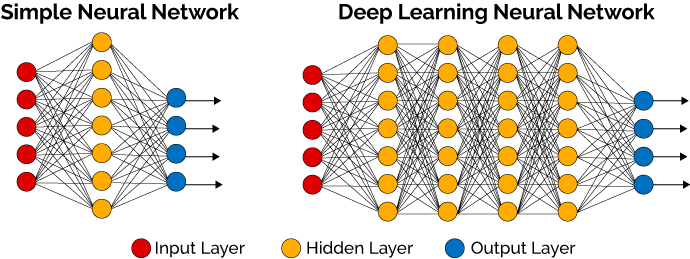
\includegraphics[width=0.8\textwidth]{img/nn_vs_dnn.png}
    \end{center}
    \caption{Primerjava zgradbe NN in DNN \cite{nn_vs_dnn}.}
    \label{img:nn_vs_dnn}
\end{figure}

Najpogosteje se za učenje nevronskih mrež uporablja algoritem vzvratnega razširjanja \emph{(ang. backpropagation)}. Algoritem se izvaja v več iteracijah, pri katerih se s pomočjo kriterijske funkcije izračuna napaka, ki je razlika med želenim izhodom in dejanskim izhodom. Napako uporabimo za izračun gradienta, ki nam pove, kako se spremeni vrednost uteži, da se napaka zmanjša. Kriterijsko funkcijo morem pravilno izbrati glede na vrsto problema, ki ga želimo rešiti. Za reševanje regresijskih problemov se najpogosteje uporablja srednjo kvadratno napako \emph{(ang. Mean Squared Error, MSE)}, za klasifikacijske probleme pa najpogosteje kategorično križno entropijo \emph{(ang. Categorical Cross-Entropy)} ali pa binarno križno entropijo \emph{(ang. Binary Cross-Entropy)}. Za iskanje optimalnih vrednosti uteži se uporabljajo različni optimizacijski algoritmi, ki na podlagi gradientnega spusta \emph{(ang. gradient descent)} iščejo minimum kriterijske funkcije. Med njimi sta najbolj znan stohastični gradientni spust \emph{(ang. Stochastic Gradient Descent, SGD)} in Adam \emph{(ang. Adaptive Moment Estimation)}.

\section{Konvolucijske nevronske mreže}
Konvolucijske nevronske mreže \emph{(ang. Convolutional Neural Network)}, so vrsta umetnih nevronski mrež, ki se pogosto uporablja v nalogah računalniškega vida, kot so prepoznavanje objektov, klasifikacija slik, detekcija obrazov in drugo. CNN modeli so tipično sestavljeni iz več ponovitev konvolucijskih slojev \emph{ang. pooling layers} in združevalnih slojev \emph{ang. pooling layers}. Za zadnjim združevalnim slojem najpogosteje sledi nekaj polno-povezanih slojev. Poenostavljena arhitektura konvolucijske nevronske mreže je prikazana na sliki \ref{img:cnn}.


\begin{figure}[htb]
    \begin{center}
        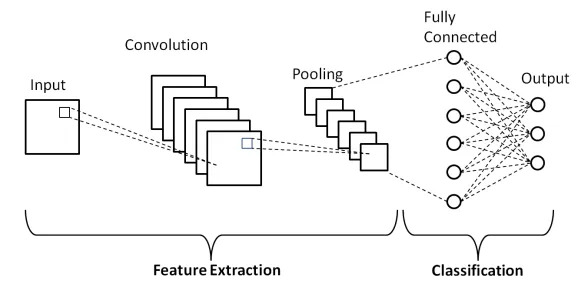
\includegraphics[width=0.8\textwidth]{img/cnn.jpg}
    \end{center}
    \caption{Poenostavljena arhitektura konvolucijkse nevronske mreže \cite{cnn}.}
    \label{img:cnn}
\end{figure}

Namen konvolucijskih slojev je pridobivanje značilk \emph{(ang. feature extraction)}, namen združevalnih slojev je zmanjševanje dimenzionalnosti podatkov, polno-povezani sloji pa so namenjeni preslikovanju pridobljenih značilk v končni izhod.

Konvolucijski sloji delujejo na principu matematične operacije konvolucije, ki je definirana na dveh funkcijah. Rezultat konvolucije nam pove, kako oblika ene spremeni obliko druge. Definirana je z enačbo:
\begin{equation}
    (f*g)(t)=\int_{\tau=-\inf}^{\inf}f(\tau)g(t-\tau)d\tau
    \label{eq:1}
\end{equation}

Kjer je \emph{f} predstavlja vhodno funkcijo, \emph{g} pa jedro konvolucije. Ker se pri obdelavi digitalnih podatkov pogosto uporablja diskretna konvolucija, je enačba \ref{eq:1} spremenjena v:
\begin{equation}
    (f*g)[t]=\sum_{k=-\inf}^{\inf}f[k]g[n - k]
    \label{eq:2}
\end{equation}

\section{Arhitektura transformer}
Transformer je arhitektura nevronske mreže, ki temelji na mehanizmu pozornosti, ki je bil predstavljen leta 2017 v članku \emph{Attention is all you need} \cite{attention_is_all_you_need}. Primarno je bila arhitektur razvita za naloge procesiranja naravnega jezika \emph{Natural language processing, NLP}, sejda pa postaja popularna tudi v drugih domenah strojnega učenja, med drugim tudi v računalniškem vidu. Osnovna arhitektura, kji je bila predstavljena v \cite{attention_is_all_you_need}, vključuje kodirni \emph{(ang. encoder)} in dekodirni modul \emph{(ang. decoder)}. Kodirnik je sestavljen iz dveh podslojev, dekodirnik pa iz treh.

\subsection{Mehanizem pozornosti}
Mehanizem pozornosti deluje na podlagi ključev \emph{(ang. key, K)}, poizvedb \emph{(ang. query, Q)} in vrednosti \emph{(ang. value, V)}. Mehanizem iz matrike ključev in matrike poizvedb izračuna matriko pozornosti. Z matričnim množenjem matrike pozornosti in matrike vrednosti dobimo linearno kombinacijo vrednosti, ki predstavljajo izhod. Razlikujemo med samopozornostjo in medpozornostjo. O samopozornosti govorim, ko če vse tri vhodne parametre dobimo iz iste množice podatkov, pri medpozornosti pa poizvedbe pridobimo iz ene množice podatkov, ključe pa iz druge.

Vhodne vektorje $ x_i, x_{i+1},..., x_{n} $ združimo v matriko $ X_{n \times d_m} $, kjer $ d_m $ predstavlja dimenzionalnost modela. Naučene parametre pa predstavljajo matrike $ W^Q_{d_m \times d_m} $, $ W^K_{d_m \times d_m} $ in $ W^V_{n \times d_m} $. Iz navedenih matrik lahko izračunamo

\begin{equation}
    \begin{split}
        Q = XW^Q, \\
        K = XW^K, \\
        V = XW^V, \\
    \end{split}
    \label{eq:3}
\end{equation}

Matrika pozornosti je definirana z enačbo:
\begin{equation}
    A(Q, K, V) = \text{softmax}(\frac{QK^T}{\sqrt{d_m}})V
    \label{eq:4}
\end{equation}

kjer funkcija \emph{softmax} spremeni vektor \emph{n} realnih števil v vektor verjetnostne porazdelitve.

Iz \ref{eq:3} in \ref{eq:4} lahko izračunamo končno izhodno vrednost mehanizma

\begin{equation}
    S = AV
    \label{eq:5}
\end{equation}


Ko se mehanizem pozornosti uporabi v dekodirnem modulu je potrebno določen del podatkov skriti. Bolj natačno, modelu je treba preprečiti, da bi lahko prejel podatke, kateri še niso bili napovedani. Skrivanje podatkov nam omogoča maska, ki določene vrednosti v matriki pozornosti \emph{A} nastavi na $ -\infty $.


\begin{figure}[htb]
    \begin{center}
        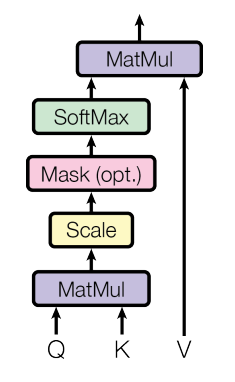
\includegraphics[width=0.3\textwidth]{img/attention.png}
    \end{center}
    \caption{Diagram izračuna pozornosti \cite{attention_is_all_you_need}.}
    \label{img:attention}
\end{figure}


\subsection{Večglava pozornost}
Da bi model lahko zajel več lastnosti vhodnih podatkov je potrebno mehanizem pozornosti nadgraditi. Večglava pozornost vzporedno izračuna več ločenih pozornosti (glav) in jih združi v končni rezultat. Vsaka glava se osredotoči na eno lastnost podatkov. Vsaka glava $ i $ ima svoje matrike naučenih uteži, končni rezultat pa se pridobi s strnitvijo posameznih matrik pozornosti.

\begin{figure}[htb]
    \begin{center}
        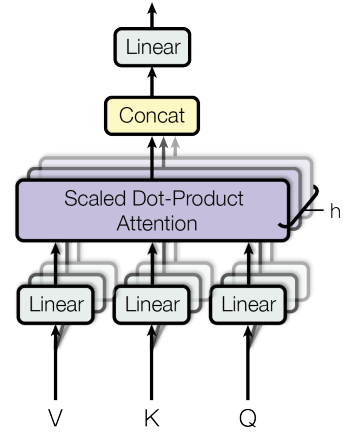
\includegraphics[width=0.3\textwidth]{img/mha.png}
    \end{center}
    \caption{Diagram izračuna večglave pozornosti \cite{attention_is_all_you_need}.}
    \label{img:mha}
\end{figure}


\subsection{Vhodna vdelava in pozicijsko kodiranje}
Preden vhodni podatki prispejo do kodirnega bloka jih je potrebno najprej pravilno predelati. Za ta namen se uporablja vdelava vhodnega niza v $ d_m $ dimenzionalni latentni prostor \emph{(ang. embedding space)}. Vhodna vdelava \emph{(ang. input embedding)} vhodne besede pretvori v vektorje, s tem model pridobi informacijo o pomenu posamezne besede. Pozicijsko kodiranje \emph{(ang. positional encoding)} pa modelu pridobi informacijo o vrstnem redu besed v nizu. Da bi se izognili velikim vrednostim v pozicijskem kodiranju, se za kodiranje uporabljata sledeči funkciji

\begin{equation}
    \begin{split}
        PE(pos, 2i) = sin(pos/10000^{2i/d_m}) \\
        PE(pos, 2i+1) = cos(pos/10000^{2i/d_m})
    \end{split}
    \label{eq:7}
\end{equation}

v enačbi \ref{eq:5} predstavlja $ pos $ pozicijo besede v nizu, $ i $ pa dimenzijo kodiranja, kar pomeni da ima vsaka dimenzija pozicijskega kodiranja pripadajočo sinusoidno vrednost.


Informacijo o pomenu in poziciji posamezne besede združimo tako, da matriki seštejemo.

\subsection{Kodirni modul}
Kodirni modul je sestavljen iz $ N $ identičnih slojev, ki so sestavljeni iz dveh pod-slojev. Prvi pod sloj je več glava pozornost \emph{(ang. multi-headed attention)} in polno povezane nevronske mreže \emph{(ang. Feedforward neural network, FFN)}.

\begin{figure}[htb]
    \begin{center}
        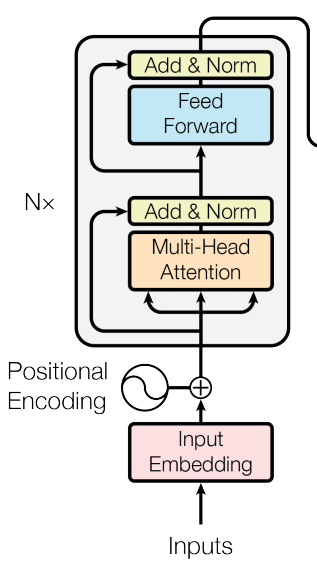
\includegraphics[width=0.3\textwidth]{img/encoder.png}
    \end{center}
    \caption{Diagram kodrinega modula \cite{attention_is_all_you_need}.}
    \label{img:encoder}
\end{figure}


\subsection{Dekodirni modul}
Dekodirni je sestavljen iz $ N $ identičnih slojev, ki so sestavljeni iz treh pod-slojev. Prvi pod sloj je več glava pozornost z možnostjo maskiranja vhodnih podatkov. Drugi pod sloj je več glava pozornost, tretji sloj pa predstavlja polno povezana nevronska mreža.


\begin{figure}[htb]
    \begin{center}
        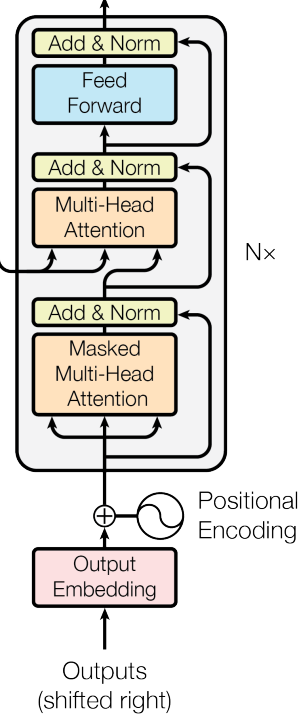
\includegraphics[width=0.3\textwidth]{img/decoder.png}
    \end{center}
    \caption{Diagram dekodirnega modula \cite{attention_is_all_you_need}.}
    \label{img:decoder}
\end{figure}

\section{Model STARK}
\label{sec:stark}
Model STARK \cite{stark} spada v družino SOT \emph{(ang. single object tracking)} sledilnikov. Primarno je sestavljen iz dveh arhitektur, konvolucijskih nevronskih mrež in arhitekture transformer, ki je bila prilagojena za vizualne sledilnike. Navdih za njegov nastanek je bil predhodni model za detekcijo DETER \cite{deter}. Ena od novosti, ki so jo uvedli v tem modelu je uporaba časovne in prostorske komponente. Prostorska komponenta vsebuje informacijo o izgledu objekta, kateremu sledi. Časovna komponenta pa nosi informacijo o spremembi pozicije objekta skozi čas.
Arhitektura, ki so jo predlagali vsebuje tri ključne elemente: kodirni modul, dekodirni modul in napovedovalno glavo \emph{(ang. predictio head)}. Kodirni modul kot vhod prejme trenutno sliko, ter matrica \emph{(ang. template)}, ki se skozi čas dinamično posodablja. \underbar{Moduli za samopozornost v kodirniku se povezave med vhodi in preko korelacije značilk}. Ker se dinamična matrica, skozi čas, posodablja, lahko kodirnik zajame tudi prostorsko in časovno informacijo o objektu, ki mu sledimo.

Prednost tega sledilnika je v tem, da ne potrebuje kompleksnega pre in postprocesiranje. Ob inicializaciji prejem kot vhod sliko in omejitveni okvir tarče. Na podlagi teh dveh vhodnih podatkov se najprej izreže ROI, ki se uporabi za izračun matrice. Ob vsaki naslednji sličici, pa so vhodni podatki slika, začetna matrica in dinamična matrica, sledilnik pa vrne izračunani omejitveni okvir.

\subsection{Arhitektura modela stark}
Arhitekturo modela lahko razdelimo na tri glavne dele: \emph{(1)} konvolucijska hrbtenica \emph{(ang. convolutional backbone)}, \emph{(2)} kodirni-dekodirni transformer in predikcijsko glavo za omejitveni okvir \emph{(ang. bounding box prediction head)}. V nadaljevanju bomo predstavili vsak od teh delov.

\subsubsection{Konvolucijska hrbtenica}
Konvolucijsko hrbtenico sestavlja model ResNet \cite{resnet}, kateremu so odstranili zadnjo sekcijo in polno povezane sloje. Kot vhod prejme hrbtenica začetno matrico $ z \in \mathbb{R}^{3 \times H_z \times W_z} $ in iskalno regijo (iz slike izrezan ROI) $ x \in \mathbb{R}^{3 \times H_x \times W_x} $. Po prehodu čez hrbtenico dobimo dve matrici značilk
$ f_z \in \mathbb{R}^{C \times \frac{H_z}{s} \times \frac{W_z}{s}} $ in $ f_x \in \mathbb{R}^{C \times \frac{H_x}{s} \times \frac{W_x}{s}} $.



%\cleardoublepage
%\addcontentsline{toc}{chapter}{Literatura}

\printbibliography[heading=bibintoc,type=article,title={Članki v revijah}]
https://www.overleaf.com/project/609ce2055f917cb2f776732e
\printbibliography[heading=bibintoc,type=inproceedings,title={Članki v zbornikih}]

\printbibliography[heading=bibintoc,type=incollection,title={Poglavja v knjigah}]

\printbibliography[heading=bibintoc,title={Celotna literatura}]


\end{document}

